%-------    CHAPTER 8     -------------------------------------------
%------ Future Improvements ----------------------------------------
\chapter{The Future}
\label{chap:future}

\begin{figure}[!h]
\centerline{\includegraphics[angle=0,height=5.5in]{Figures/Chap8/Porcupine.png}}
\end{figure}
\clearpage



%------------------------------------------------------------------------------
\section{Possible Future Improvements}

At present none of the three interferometers operates at the designed sensitivity
level. In addition, the duty cycles (especially of the Livingston detector) are
not at the 90\% level which they were designed for. The following are some ideas
for improving the state of affairs. Some are currently being explored and some only
exist on paper.


\subsection{Seismic Isolation}
During the course of this writing, a scheme has been developed for mitigating the
excess seismic noise which limits the duty cycle and data quality of the Livingston
interferometer.

Quiet hydraulic actuators~\cite{Giaime:AdvIso} with collocated sensors are being 
installed on the existing seismic isolation support structure. This system,
the Hydraulic External Pre-Isolator (HEPI), is also intended for the Advanced LIGO upgrade.

Since the in-vacuum, passive isolation stack has various cross-couplings (e.g. from
pitch to horizontal motion), the HEPI is designed to reduce the vibration in all 6
DOF on the outside of the vacuum chamber. Preliminary testing indicates that the
HEPI performance will exceed the factor of 5-10 reduction in broadband displacement
noise which was the goal.

The Hanford site seems to be sufficiently quiet (with the exception of occasional
periods of high winds), such that at present, no such drastic retrofit is planned.
However, the dramatic success of HEPI could make the Hanford sites ground noise
seem egregiously large in comparison to the isolated Livingston platforms.


\subsection{Output Mode Cleaner}

The current interferometers have many problems associated with poor beam quality or
imperfect interference at the interferometer's dark port:

\begin{itemize}
\item Excess carrier light at the dark port produces excess shot noise.

\item The reflectivity difference of the two arms will produce a static, TEM$_{00}$,
      carrier field at the dark port. This static field beats with noise on the
      sideband light to produce noise in the signal channel.

\item The portion of the sideband field which does not spatially overlap with
      the carrier does not contribute to increasing the optical gain. Instead,
      it produces many junk effects: shot noise, acoustic sensitivity, jitter
      sensitivity, etc.
\end{itemize}

One solution to these problems which is being currently pursued is the use of an
output mode cleaner. This would be a short, rigid, triangular cavity placed on
the anti-symmetric port output table. Such a short ($\sim$5 cm), low 
($\sim$ 30) finesse cavity would have large enough linewidth to transmit the 
RF sidebands and the carrier in the same resonance. Higher order spatial modes, 
however, would be passively rejected just as in the input mode cleaners. 
The suppression of the higher 
order spatial modes is given by Equation~\ref{eq:ModeCleaning}.

Once the the contrast defect due to higher order modes has been effectively
removed, one can re-optimize the SNR by adjusting the modulation depth for
the resonant sidebands as described in Section~\ref{sec:darksignals}.


\subsection{Thermal Compensation}
\label{sec:ThermalComp}

A serious problem with the interferometers is the unstable nature
of the power recycling cavity. 

The power absorbed by the optics forms a thermal lens in the bulk of the glass
through the temperature dependence of the index of refraction. The original design 
planned on a precise amount
of thermal lensing and pre-polished the power recycling mirror to account for this.
Preliminary estimates indicate that the absorption levels vary substantially
from optic to optic. 

The carrier mode in the recycling cavity is determined by the average spatial mode
of the arms and so the carrier field is largely immune to curvature errors in the
recycling cavity. The sideband fields are not resonant in the arms and so the
mode matching of the sideband to the recycling cavity depends critically on the
amount of thermal lensing. The experience with the interferometers so far has
shown that it will be necessary to control the recycling cavity resonant mode
to keep it well matched to the arms. 

The three most deleterious consequences of the unstable recycling cavity are:

\begin{itemize}
\item The RF sideband is not spatially mode-matched to the recycling cavity. 
      So most ($\approx$90-95\%) of the sideband power is reflected from the
      recycling cavity. This
      results in low optical gain at both the recycling cavity pickoff and 
      anti-symmetric ports.

\item The RF sideband field which does make it to the AS port does not overlap
      well with the carrier field and therefore the gravitational wave signal sidebands. This
      means that much of the RF sideband field which is there contributes 
      to increased shot noise and not to the signal strength.

\item The unstable nature of the PRC results in large optical gain modulation
      for small angular fluctuations. This leads to instability in all of the
      conditionally stable servo loops.
\end{itemize}

To compensate for the lack of thermal lensing, a system, initially intended
for Advanced LIGO~\cite{Ryan:Thesis}, is being commissioned to
stabilize the cavity. By applying the correct spatial distribution of heat 
to each ITM, one can induce a thermal lens in the test mass bulk. This will
pull the recycling cavity from unstable to marginally stable. 

The plan is to heat each ITM with a CO$_2$ laser with a fixed mask to shape 
the heat distribution. The Nd:YAG laser power will be turned up all the way 
and the CO$_2$ beam will be adjusted accordingly to maximize the SNR of the
$\delta L_{-} \rightsquigarrow AS\_Q$ readout.


\subsection{Oscillator Phase Noise}

During the course of commissioning, a strange and large sensitivity to phase
noise on the RF oscillator was measured. This noise source dominates the 
interferometers' noise budgets above 1 kHz.

While the source of the coupling is not established as of yet, it is believed
that reducing the phase noise of the oscillator itself will partially
mitigate the problem. In the near future low noise, crystal oscillators will
be installed. These oscillators have a narrow tuning range compared to the
existing frequency synthesizers, but have a SSB phase noise of -165 dBc/$\sqrt{\mbox{Hz}}$
at 1 kHz (as compared to the -150 dBc/$\sqrt{\mbox{Hz}}$ of the currently installed units).


\subsection{Laser Frequency Noise}

\subsubsection{A Better Frequency Reference}
As shown in Figure~\ref{fig:CMnoise}, the overall frequency stabilization
factor would be almost good enough except that the noise in our frequency
noise readout channel is too high to produce a quiet laser beam. The main
work that needs to be done is to reduce the shot noise limited sensitivity
at that port.

Until now we have been using a signal readout scheme where each length
signal is constructed by demodulating at the resonant sideband frequency.
Unfortunately, this causes us to suffer problems similar to those experienced
at the AS port with junk light. The uncontrolled Q phase signal in reflection
dominates, by a few orders of magnitude, the I phase signal used to readout
the $L_{+}(f)$ or $\nu(f)$ signal. This limits the total amount of light we can
detect without saturating the RF photodetector. At such low levels ($\sim$1 mA,
30X smaller than designed) the shot noise limit is quite high.

An alternative scheme is to use the non-resonant sideband (which is already used
for angular sensing). Whereas the resonant
sideband level at the reflected port is slowly extinguished as the recycling
cavity is thermally lensed, the non-resonant sideband is, in principle, unaffected
by the state of the recycling cavity and can produce a strong signal, largely
independent of the problematic recycling cavity. There is also no Q phase signal 
expected at the non-resonant sideband frequency, in principle.

\subsubsection{More Loop Gain}

Above a few kHz, the frequency noise exceeds its designed noise level. The result
is that the interferometer sensitivity would be compromised at high frequencies
once the other noise sources are reduced.

The reason for this high frequency excess is that early in the commissioning phase
for the Mode Cleaner, the servo loop gain was reduced to make the servo more
stable. In this low gain state the VCO phase noise dominates the MC noise 
(see Figure~\ref{fig:MCnoise}) and this propagates into the interferometer.

Some combination of higher loop gain in the MC and a quieter VCO will have to
be explored in the future to meet the noise requirements.


\subsection{Wavefront Sensing}
\label{sec:WFSfuture}

At the time of this writing, the full Wavefront Sensing (WFS) and angular control
system has been demonstrated to work on all the interferometers, although it
has only stably operated on the Hanford interferometers.

In order to have some day to day stability and consistent data quality, it is
vital that this system work on all interferometers. In the near future it is
envisioned that the WFS system will be commissioned in Livingston to bring it
to the level of the Hanford instruments.

On all the interferometers, there remains substantial work to be done on the
electronics for this system to reduce the noise contributed to the gravity
wave channel. The reduced noise will allow operation with higher gain. 
There does not seem to be any fundamental roadblock here.


\subsection{Increased Laser Power}

In the past few years of detector commissioning, the laser power into the
interferometer has been run, usually, at lower power than designed for. 
This is due to a number of reasons:

\begin{itemize}
\item Low transmission through the optics between the laser and the interferometer.
\item Unintentional low power due to degraded Power Amplifier pump diodes, poor amplifier
      alignment, or low power from the master oscillator.
\item Intentional low power from the laser by lowering the pump diode current to extend
      diode lifetime.
\item Not being able to handle high power in the interferometer itself (scattering,
      radiation pressure, wimpy photodetectors, etc.)
\end{itemize}

Efforts are now underway to chip away at this power deficit by better alignment,
mode-matching through the PMC, increased pump power, etc. It looks promising that
there soon can be the full 6 Watts of power entering the interferometer.

A hypothetical question to pose is, what can be done to further increase the
laser power by another factor of 2-5. Some concepts to quantitatively explore
over the next two years are:

\begin{itemize}
\item Increase the power output of the master oscillator. Currently we are
      pumping the NPRO master oscillators at $\sim$500 mW. At this power level
      the PA is only partially saturated and so while doubling the MO power
      will not double the MOPA power, we should explore how much this will give.

\item Add another amplifier. By taking the MOPA output and putting it through
      a single pass, commercially available amplifier or another double-pass
      PA like we have now would make a much more powerful laser; a MOPAPA.

\item Convert the PA into a ring cavity and injection-lock it to the NPRO.
\end{itemize}

\subsection{Low Noise DAC}

The noisy digital-to-analog converters currently used require us to use
aggressive, complex analog filtering to both achieve low displacement noise
and yet have enough range to accomodate the low frequency seismic noise.

The development and testing of DACs with $\sim$30X less noise is being
pursued. These would lower the influence of DAC noise below the SRD/10 level
in all interferometers and also allow one to rework the post-DAC filtering
to give increased dynamic range.

\subsection{Sweet Spot on the Suspension}
\label{sec:sweetspot}

The estimate made for suspension thermal noise in Section~\ref{sec:SUSthermal}
assumed that the beam was centered on the test mass. This is not the position
in which the suspension thermal noise is minimized.

It was recognized several years ago \cite{Gaby:Thermal,Levin:SUSthermal} that 
there is a 'sweet spot' on the
optic which minimizes the thermal noise. When the test mass pendulates, most
of the loss is due to bending in the wire at the top suspension point and at
the bottom of the wire, near where it contacts the optic (see Figure~\ref{fig:SUS}). 
By symmetry, only the thermal forces generated at these two points affects the 
test mass motion.


For the thermal forces generated at the bottom of the wire, there is a node
in the optics motion slightly below the center of mass. By adjusting the cavity
axis so that the beam resonates at this point, one can make the measured
interferometer strain noise insensitive to the this thermal noise and only
sensitive to the loss in the top of the wire.

Following the method of \cite{Gaby:Thermal} we can get a numerical result and
find that the minimum is $\sim$1 cm below the center of mass. In the case where
suspension thermal noise is the only noise in that band we can get a $\sim$20\%
reduction from $\sim$50-100 Hz.


\subsection{Low internal mode noise}

Between the time the interferometers were designed and the present, the state-of-the-art
in thermal noise modeling has crept forward somewhat. In particular, it has been
recognized that the substrate thermal noise should be less than what was assumed
in the initial design and that coating thermal noise is approximately equal to
the substrate thermal noise for the LIGO-I choice of beam parameters and coating
materials.

In particular, it appears that the overall test mass thermal noise will come out
$\sim$2X smaller than was expected originally.
 

\subsection{DC Readout}
\label{sec:DCreadout}

In the current signal readout scheme, the GW signal is encoded as 
an amplitude modulation on the RF carrier (which is itself generated as a
beat between an optical frequency carrier and an RF sideband). This method
has a historical origin; in the 20$^{th}$ century, the amplitude and
phase noise on commercial lasers was so bad that there was no hope of
reaching the shot noise limit at the audio frequencies where GW's are
expected.

Recently~\cite{Peter:DCreadout} it has come to light that this is no 
longer the case. The combination of quiet, solid-state lasers with
the high-gain, low noise, amplitude and frequency stabilization servos
already significantly reduces these noises. The advantage to eliminating
the RF sidebands, however, is revealed through the way the laser noise
couples into the interferometer. As described in Sections
\ref{sec:IntensityNoise} and \ref{sec:FreqNoise}, the RF sidebands do
not experience the $\sim$1 Hz low pass filter of the full coupled
cavity resonance that the carrier does and so eliminating them
would reduce the coupling from laser amplitude and frequency noise
and of course, completely eliminate oscillator based noises.

Instead of reading out the signal by doing a phase modulation on the
input beam, one can just shift the differential arm length slightly,
yielding a first order change in the AS port power as a function of
differential arm length.

There are a few other advantages to employing a DC readout:

\begin{itemize}
\item Exploring the possible space of modulation/demodulation waveforms
      \cite{Meers:modulation}, we know that the theoretical best SNR
      is achieved by using no modulation or demodulation. 

\item Even better than the fact that it is the theoretical best, is the
      fact that it guarantees perfect overlap between the local oscillator
      and signal fields: The 'LO' in this case is just the static
      carrier generated by the intentional arm length offset.

\item Instead of all of the complicated electronics associated with an
      RF readout, one can just readout the DC power on the photodiode.
      With an Output Mode Cleaner this requires only a few mW total.
\end{itemize}




\section{Estimating the future performance}

In the past, predictions about the detectors' noise performance have had a mixed
level of accuracy. It is certainly true, however, that the predictions have gotten 
more accurate as the noise is reduced and the instrumental characterization becomes
more advanced.

Determing the ultimate sensitivity of the detectors is of great interest, since
we would like to know sooner than later if some major upgrade or redesign will
be required to reach the design sensitivity.

The initial LIGO design curve was made $\sim$15 years ago, based upon the
knowledge available at that time. Now that the interferometers are built we
are able to make more accurate estimates of many of the parameters involved
in generating these noise curves. There are three particularly important cases:

\begin{itemize}
\item The initial design noise curve was dominated at the $\sim$150 Hz minimum
      by thermal noise in the mirrors. The loss in the mirrors appears to be 
      10X less than expected. This makes the thermal noise from the mirror 
      substrate 3X less than the design.

\item The interferometers' contrast defects are all 20-100X better than the
      conservative estimate made in the design. This gives a reduced level of
      shot noise which dominates above 200 Hz.

\item After the initial design, it was recognized that the true mechanism for
      suspension thermal noise gave a steeper frequency dependence and so the
      suspension thermal noise contribution is much less above the pendulum
      resonance frequency.
\end{itemize}

As shown in Figure~\ref{fig:S5noise}, I predict that the sensitivity of the initial
interferometers will significantly surpass the design, as long as we are able to
reduce the technical noise sources to their initial design levels and no
unforseen, insurmountable noise sources are discovered.

 
\begin{figure}[!h]
\centerline{
  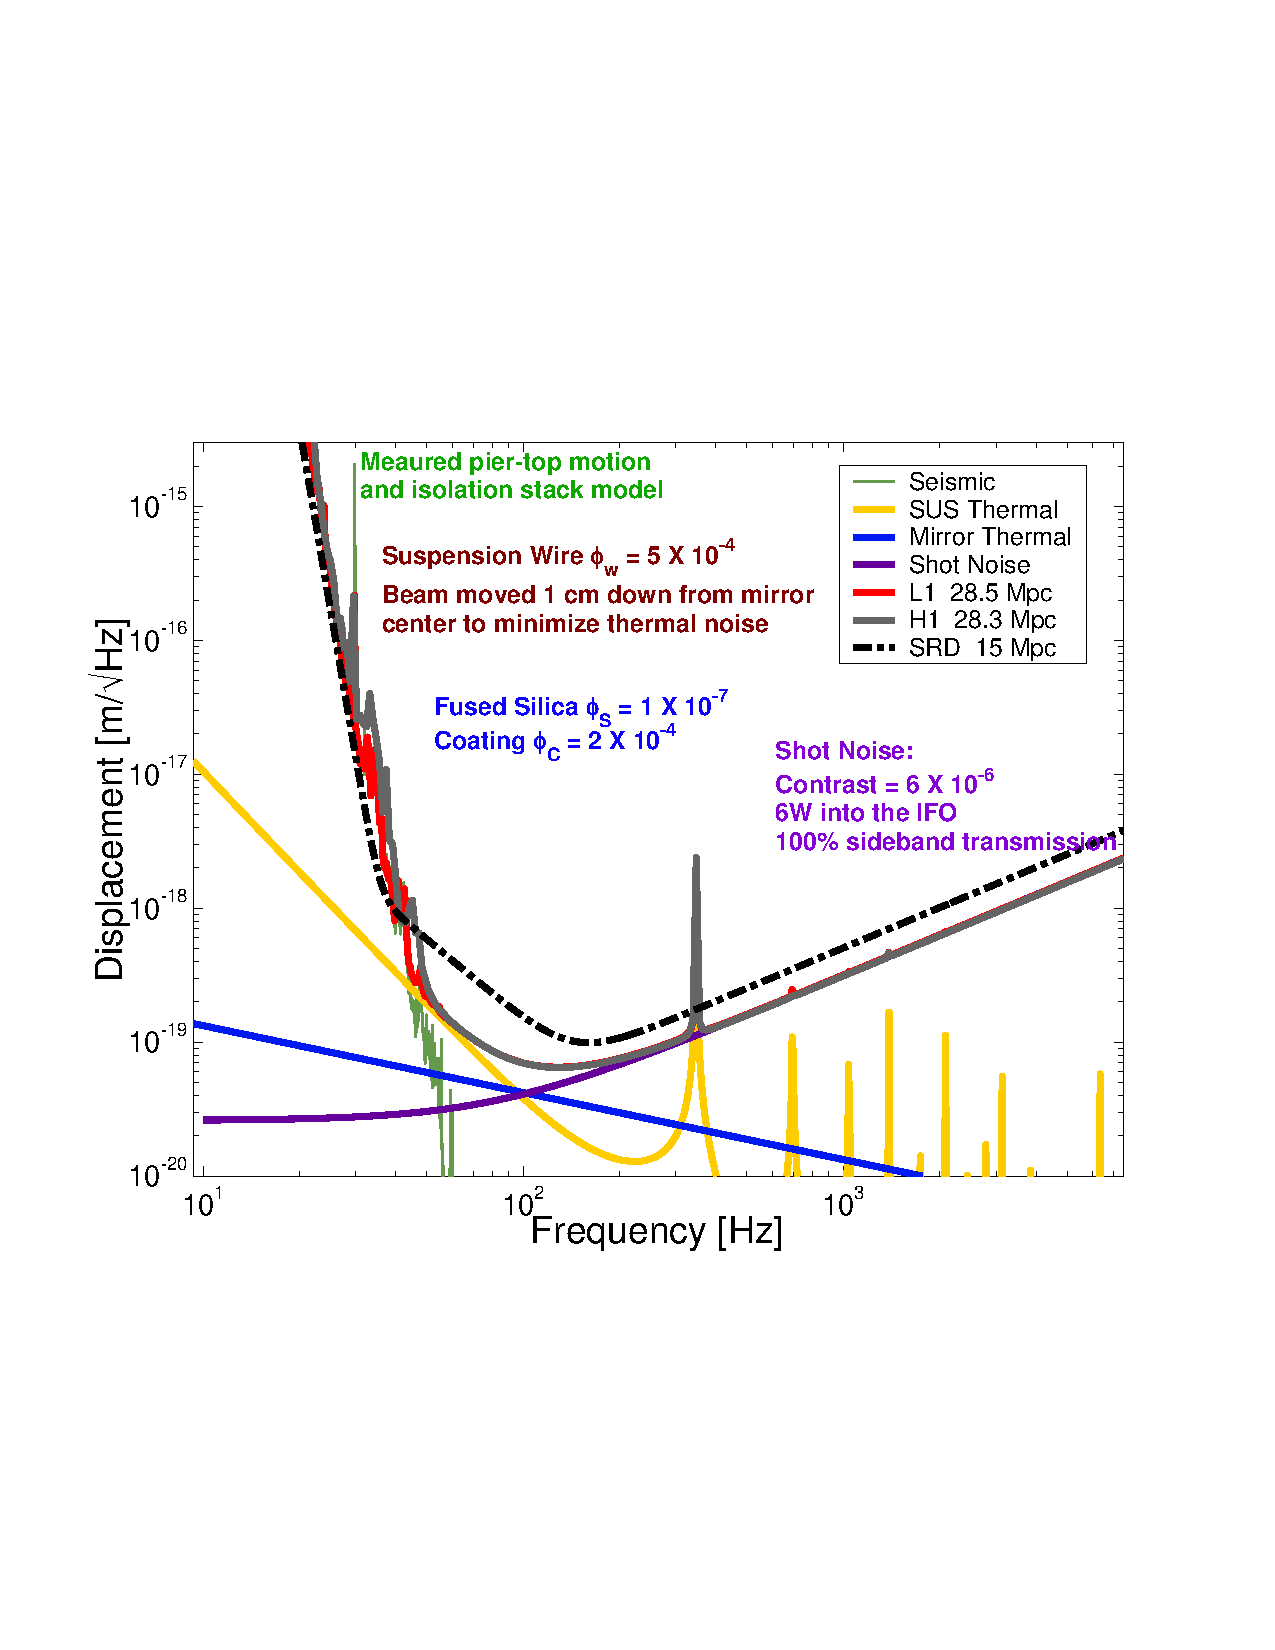
\includegraphics[angle=0,width=6.5in]{Figures/Chap8/s5noise2.pdf}}
\caption[S5 Noise]{Best possible noise curve using the existing IFO components. The significant
                   sensitivity improvements from using a DC readout and higher laser power
                   are not shown.}
\label{fig:S5noise}
\end{figure}



